%%% 関西大学 総合情報学部 松下ゼミ 進捗報告 TeXテンプレート Ver 1.1 (2011/12/04) %%%
\documentclass{matsushita-zemi}
\usepackage[dvipdfmx]{graphicx}
\usepackage{comment}
\graphicspath{{./fig/}}

%%% タイトル (長くなる場合は¥¥で適宜改行すること)%%%
\title{HogeHogeにおけるHogeに関する研究}

%%% 氏名 (姓・名の間は半角スペース) %%%
\author{内藤 峻}

\begin{document}
\maketitle

%%% 以下、本文 %%%
\section*{概要}
\label{abstract}
ネットワーク上には多様な種類の情報が存在しており、それらをユーザの要求に応じて適応的にまとめ上げる技術が渇望されている。その一つとして、テキストなどの言語情報と統計データ等の数値情報の相補的な利用に関する研究を行っている。その一環として、本研究では言語情報と数値情報が密接な関係にある株価などの動向情報に着目しそれらを統一的な枠組みで可視化する手法を提案する。株価などの統計情報の場合、その正確な値を知るには数値情報が適切であるのに対して、変動の大局的な理解や背景となる事象の把握には言語情報が適している。そこで、これらを一つのグラフ上に提示し、その情報源に対話的にアクセスできるようにした。\cite{Elucignage}\cite{Elucignage-jsai}\cite{information_compilation}\cite{Tagged_corpus}

\section{はじめに}
\label{background}
%電子化が普及している話
%それらの情報を利用して意思決定や問題解決に役立てられている話
%しかし、情報は膨大になっている、時間にともなって更に増加を続けている話
%それらをまとめる技術が求められている話
%しかし、情報には様々な種類がある話
%本提案では数値情報(統計データ)と言語情報(新聞記事)に着目した話
近年、様々な情報が電子化されネットワーク上に蓄積されている。それに伴い、これらの情報を利用して意思決定や問題解決に役立てる試みがなされている。しかし、蓄積された情報は膨大なっていうるえ、時間の経過に伴って更に増加を続けている。そのため、ユーザの関心や興味に合致する情報に直感的かつ簡便にアクセスするための技術が求められている\cite{基盤技術}\cite{可視化手法}。情報にはテキスト、画像、音声、動画と様々な種類がある。このような要求に答える技術のひとつとして、本提案では統計データ等の数値情報と新聞記事等の言語情報に着目した。

本稿の構成は以下の通り。まず、デザイン指針について述べる。その後、プロトタイプを説明し、続いて、先行研究を示す。

\section{デザイン指針}
%目的をどのように達成するのかという話
%どのような機能が必要なのか?何故必要なのか?
%シナリオに基づいた話

\section{Elucignage プロトタイプシステム}
\subsection{概要}
ユーザの関心がある動向情報を時系列数値情報を用いて統計グラフとして描画し、そのグラフの要因となる記事をその内容に適したアイコンの形式で提示する方法を採用する。このアイコンは要因となる記事のアクセスを可能にする。これにより、ユーザは統計グラフの外観を理解するだけでなく、興味を持った箇所についてどのようなことが述べられているかをその要因となる記事にアクセスすることで参照できる。また、記事の一部を画面の一部に表示し、そこからグラフのどの部分に該当しているかを示す機能を備える。これにより、要因となる記事がグラフのどの部分で記述されたものであるかを確認できる。
\subsection{実装}
\begin{comment}
%サンプル
現在、図\ref{LTCond} ならびに図\ref{LCDCond} に示すような二つの実験環
境を作成し、表\ref{exp} に示す 4 群を対象に、被験者間実験をデザインし
ている。実験課題には、迷路上で 1 名の逃亡者を 3 名の追跡者が追いかけて
捕まえるタイプの課題(迷路課題)を用いる。現在、本課題のプログラムを 
Processing で作成しており、クライアント部が完成、サーバ部も 8 割の実装
が完了している。8 月末までにサーバ部を実装し、テストトライアルを行うと
ともに、その結果を反映させた改良を行う。その後、ゼミ外から被験者 80 名
を募集し、本実験を行う。本実験は9月から10月を予定している。
\end{comment}

\section{先行研究}
\label{relatedworks} 
動向情報を可視化する枠組みとして、山本らの可視化システム\cite{タグ付きコーパス}や松下らのSTEND\cite{STEND}、蓮井らのグラフ型インタフェース\cite{比較}、加藤らの視覚オブジェクト\cite{情報編纂研究会}などがある。

山本らは、動向情報の変化要因に関する重要語を注釈としてグラフに表示する方法を提案している(図\ref{system})\cite{タグ付きコーパス}。要因の抽出では、動向情報が記載された新聞記事と文章の類似度が高い新聞記事を要因としている。また、要因とされた新聞記事からのキーワード抽出は、1月分の新聞記事を1ドキュメントとみなしたTF・IDF値に基づき行っている。動向情報とその要因の表示方法に関するアンケート調査からは、ユーザが動向情報に関する要因を知りたいことは、動向情報を示したグラフ中の変化が大きい部分とその前後、最大位置と最小位置、及び最初と最後の3つに分類できることが分かったと述べられている。また、要因の表示方法としては、1ウィンドウに3つ程度のトピックを簡潔に示したものや、要因をタイトルやキーワードとともに表示すれば良いことが分かったと述べられている。
\begin{figure}[tb]
  \begin{center}
   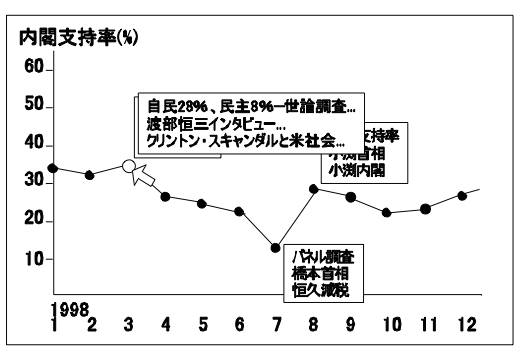
\includegraphics[width=8cm,bb=0 0 521 356]{tagu.PNG}
  \end{center}
 \caption{システムの出力例}
 \label{system}
\end{figure}
%%%この方法は本稿の提案方法と問題意識が近く、特に情報提示に関しては参考になる点も多い。しかし、その情報提示がユーザとのインタラクションにおいてどのように作用し適応していくかについては、現状ではあまり深く検討されていない。本提案はユーザのインタラクションに基づく適応的情報提示に大きな関心があり、この点でこれらの方法と方向性が異なる。%%%

松下らは、グラフ概形を示唆するシステムSTENDを提案している\cite{STEND}。STENDは時系列数値情報を扱わず、新聞記事のテキストデータのみから取得可能な数値情報と定性情報に着目してグラフ描画を試みたものである(図\ref{STEND})。テキスト中の「昨年10月より約40%の下落になっている」「前年同月に比べて5ドル上昇した」等の比較表現や「安定傾向にあった」「10月をピークに下落している」等の定性表現から情報を抽出している。情報提示では、統計グラフを用いず数種類の点や短形、形状の異なる幾つかの矢印記号を組み合わせることでその代替を試みている。

%%%松下らは、グラフ概形を示唆するシステムSTENDを提案している。STENDは時系列数値情報を扱わず、新聞記事のテキストデータのみから取得可能な数値情報と定性情報に着目してグラフ描画を試みたものであり、本提案とは力点が異なる。テキスト中の「昨年10月より約40%の下落になっている」「前年同月に比べて5ドル上昇した」等の比較表現や「安定傾向にあった」「10月をピークに下落している」等の定性表現から情報を抽出している。情報提示では、統計グラフを用いず数種類の点や短形、形状の異なる幾つかの矢印記号を組み合わせることでその代替を試みている。
\begin{figure}[tb]
  \begin{center}
   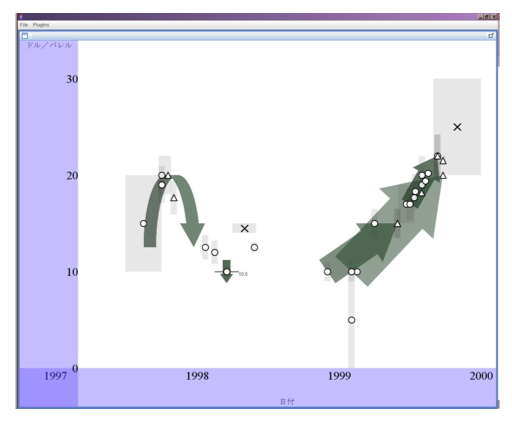
\includegraphics[width=8cm,bb=0 0 512 422]{STEND.PNG}
  \end{center}
 \caption{STENDの描画例}
 \label{STEND}
\end{figure}
%%%コピペ%%%
%%%テキストの動向情報を対象とした可視化%%%

%%%蓮井らは、複数の動向情報を比較するグラフ型インタフェースを提案している。%%%
蓮井らは、動向情報データを対象に、異なるデータ同士の比較とそれに関する詳細な情報へのアクセスの支援を目指したグラフ型インタフェースを提案している\cite{比較}。2つのグラフがあり、片方のグラフをドラッグ&ドロップすることにより、比較を実現している。また、このような比較行為によって生じるユーザの興味のきっかけによる取り組みを円滑に行うため、詳細な情報へのアクセスを可能にしている。実験結果から、詳細なアクセス手段は有望であることと重ね合わせによる比較分析手法に有望性があることが述べられている。
%%%コピーが多い%%%
%%%※STENDの未解決問題%%%
%%%具体的に書きすぎ、軽くで良い%%%

加藤らは、グラフに文章を関連付けた視覚オブジェクトを提案している。2つの画面を上下に配置しており、上画面にグラフ概形(図\ref{oblject}上画面)、下画面に状況記述を表現している(同下画面)。また、下画面ではグラフ上のアイコンに対応する記事の一部が表示されている。この記事とグラフは一方を選択すると他方の対応する部分がハイライトする等の対応付けがなされている。
さらに、視覚オブジェクトの操作として、グラフ表示を操作するためのパネルがグラフの右下に配置されている。これを使って、表示する期間の変更や、拡大縮小が行える。そのため、これらの視覚オブジェクトを介して特徴点や文書の閲覧が行われる必要があるとされている。これら全般を扱うインタラクションの設計が必要となると述べられている。
\begin{figure}[tb]
  \begin{center}
   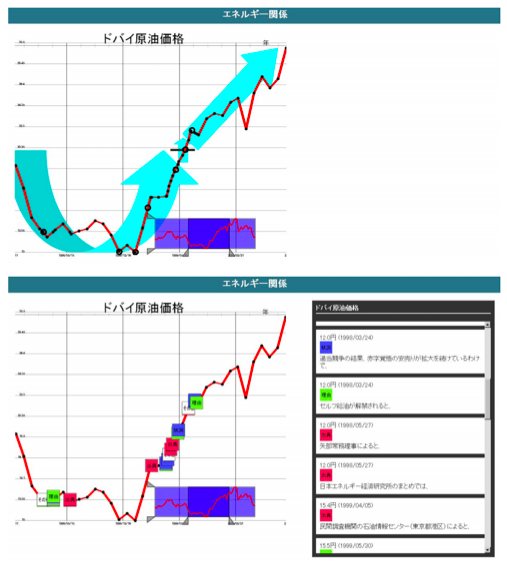
\includegraphics[width=8cm,bb=0 0 507 566]{object.PNG}
  \end{center}
 \caption{文章とグラフを関連付けた視覚オブジェクト}
 \label{oblject}
\end{figure}

%%%少なすぎる%%%

\section{おわりに}

\begin{comment}
%サンプル
%% 図の挿入 (captionが下)
\begin{figure}[b]
 \centering
 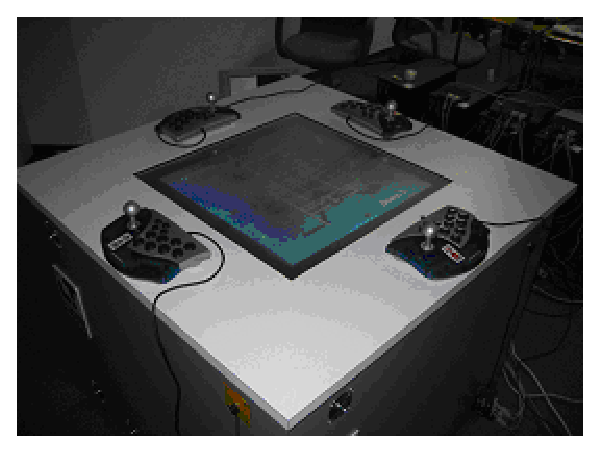
\includegraphics[width=0.4\columnwidth]{LTCond.eps}
 \caption{Lumisight Table 条件}
 \label{LTCond}
\end{figure}

\section{先行研究}
\label{relatedworks} 

%% 表作成 (captionが上)
\begin{table}[p]
\caption{実験群}
\label{exp}
\begin{center}
\begin{tabular}{lcc}
\hline\hline
         & 統制群 1 & 統制群 2\\
\hline
LT 条件  & 20       &   20    \\
LCD 条件 & 20       &   20    \\ 
\hline
\end{tabular}
\end{center}
\end{table}
\end{comment}

%%% 参考文献 %%%
\bibliographystyle{ipsjunsrt}
\bibliography{reference}

\end{document}